% This is based on "sig-alternate.tex" V1.9 April 2009
% This file should be compiled with V2.4 of "sig-alternate.cls" April 2009
%
\documentclass{report}

\usepackage[english]{babel}
\usepackage{graphicx}
\usepackage{tabularx}
\usepackage{subfigure}
\usepackage{enumitem}
\usepackage{url}


\usepackage{color}
\definecolor{orange}{rgb}{1,0.5,0}
\definecolor{lightgray}{rgb}{.9,.9,.9}
\definecolor{java_keyword}{rgb}{0.37, 0.08, 0.25}
\definecolor{java_string}{rgb}{0.06, 0.10, 0.98}
\definecolor{java_comment}{rgb}{0.12, 0.38, 0.18}
\definecolor{java_doc}{rgb}{0.25,0.35,0.75}

% code listings

\usepackage{listings}
\lstloadlanguages{Java}
\lstset{
	language=Java,
	basicstyle=\scriptsize\ttfamily,
	backgroundcolor=\color{lightgray},
	keywordstyle=\color{java_keyword}\bfseries,
	stringstyle=\color{java_string},
	commentstyle=\color{java_comment},
	morecomment=[s][\color{java_doc}]{/**}{*/},
	tabsize=2,
	showtabs=false,
	extendedchars=true,
	showstringspaces=false,
	showspaces=false,
	breaklines=true,
	numbers=left,
	numberstyle=\tiny,
	numbersep=6pt,
	xleftmargin=3pt,
	xrightmargin=3pt,
	framexleftmargin=3pt,
	framexrightmargin=3pt,
	captionpos=b
}

% Disable single lines at the start of a paragraph (Schusterjungen)

\clubpenalty = 10000

% Disable single lines at the end of a paragraph (Hurenkinder)

\widowpenalty = 10000
\displaywidowpenalty = 10000
 
% allows for colored, easy-to-find todos

\newcommand{\todo}[1]{\textsf{\textbf{\textcolor{orange}{[[#1]]}}}}

% consistent references: use these instead of \label and \ref

\newcommand{\lsec}[1]{\label{sec:#1}}
\newcommand{\lssec}[1]{\label{ssec:#1}}
\newcommand{\lfig}[1]{\label{fig:#1}}
\newcommand{\ltab}[1]{\label{tab:#1}}
\newcommand{\rsec}[1]{Section~\ref{sec:#1}}
\newcommand{\rssec}[1]{Section~\ref{ssec:#1}}
\newcommand{\rfig}[1]{Figure~\ref{fig:#1}}
\newcommand{\rtab}[1]{Table~\ref{tab:#1}}
\newcommand{\rlst}[1]{Listing~\ref{#1}}

% General information

\title{Multiplayer Pac-Man\\
\normalsize{Distributed Systems -- Project Proposal}}
\subtitle{subtitle}

% Use the \alignauthor commands to handle the names
% and affiliations for an 'aesthetic maximum' of six authors.

\numberofauthors{6} %  in this sample file, there are a *total*
% of EIGHT authors. SIX appear on the 'first-page' (for formatting
% reasons) and the remaining two appear in the \additionalauthors section.
%
\author{
% You can go ahead and credit any number of authors here,
% e.g. one 'row of three' or two rows (consisting of one row of three
% and a second row of one, two or three).
%
% The command \alignauthor (no curly braces needed) should
% precede each author name, affiliation/snail-mail address and
% e-mail address. Additionally, tag each line of
% affiliation/address with \affaddr, and tag the
% e-mail address with \email.
%
% 1st. author
\alignauthor \normalsize{Stefan Oancea, Johannes Beck}\\
	\affaddr{\normalsize{ETH ID-1 14-944-912, ETH ID-2 14-805-279}}\\
	\email{\normalsize{oanceas@student.ethz.ch, beckjoh@student.ethz.ch}}
\alignauthor \normalsize{Markus Hauptner, Florian Morath}\\
	\affaddr{\normalsize{ETH ID-3 13-939-871, ETH ID-4 14-931-968}}\\
	\email{\normalsize{markuhau@student.ethz.ch, fmorath@student.ethz.ch}}
\alignauthor \normalsize{Linus Fessler, Tiziano Zamaroni}\\
	\affaddr{\normalsize{ETH ID-5 14-924-203, ETH ID-6 XX-XXX-XXX}}\\
	\email{\normalsize{fesslerl@student.ethz.ch, ztiziano@student.ethz.ch}}
}



\begin{document}

\maketitle

\section{Introduction}

%------------------------------------INTRODUCTION------------------------------------

Since 1980, the game Pac-Man has fascinated players around the world. 
Starting as an arcade game, it was adapted for many platforms while technology was improving and is still played today on mobile devices.
While graphics have improved significantly over time and new features were added to the original idea of the game, there is still a major drawback to most of its versions as the game only provides single player user experience.

 
Our goal is therefore to exploit the opportunities of modern mobile devices in order to create a new user experience. 
This new user experience will consist of the well known Pac-Man game combined with a distributed multiplayer approach.
The idea will be implemented as an Android application allowing the user to create a new instance of the game by starting a server on an Android device. 
Other users can then connect to this server with their own devices.



\section{System Overview}

%-----------------------------------SYSTEM OVERVIEW----------------------------------
Figure 1 gives an overview of the Pacman app Activities.
The app starts in the Main activity. 
Here, the user can choose to either edit the game settings, host or join a game by pressing corresponding buttons.

If the user presses the "Settings" button, the app will switch to the Settings Activity, where the device`s local IP address is listed and the following properties can be changed:
\begin{enumerate}
	\item The username that will be used in the game.
	\item The port on which the local server would listen to.
	\item The IP address and port on which the app would try to connect to a server.
\end{enumerate}

If the user chooses the "Host" button, the app will switch to the Lobby Activity (Host).
Here, the user can await new clients and see which ones are currently connected (identified by usernames).
Furthermore, the user can decide to start the game by pressing a "Start" button.
This will launch the Game Activity and start the actual game.

If the user chooses the "Join" button, the app will switch to the Lobby Activity (Client).
Here, the user can see the host's username and which clients are currently connected (identified by username).
In contrast to the host's view, the client can not see a "Start" button, but instead has to wait for the host to start the game.

Once the game started, a Score activity keeps track of the current performance of the players. 
The game will be played in rounds, such that every player plays as Pac-Man once. 
If Pacman manages to take all the points that are positioned on the map or looses all his available lifes, the game ends and the player roles (who plays which figure) will be distributed anew. Furthermore, a timer will keep track of the time played and end the game if a certain time has been reached.

Independent from the device's role as host or client, the app will automatically switch to the Score Activity after the game has ended.
This Activity displays each users score (determined by the gameplay performance).
The only following action is to return to the Main Activity by pressing a button. 
 
\begin{figure} [ht!]
	\centering
    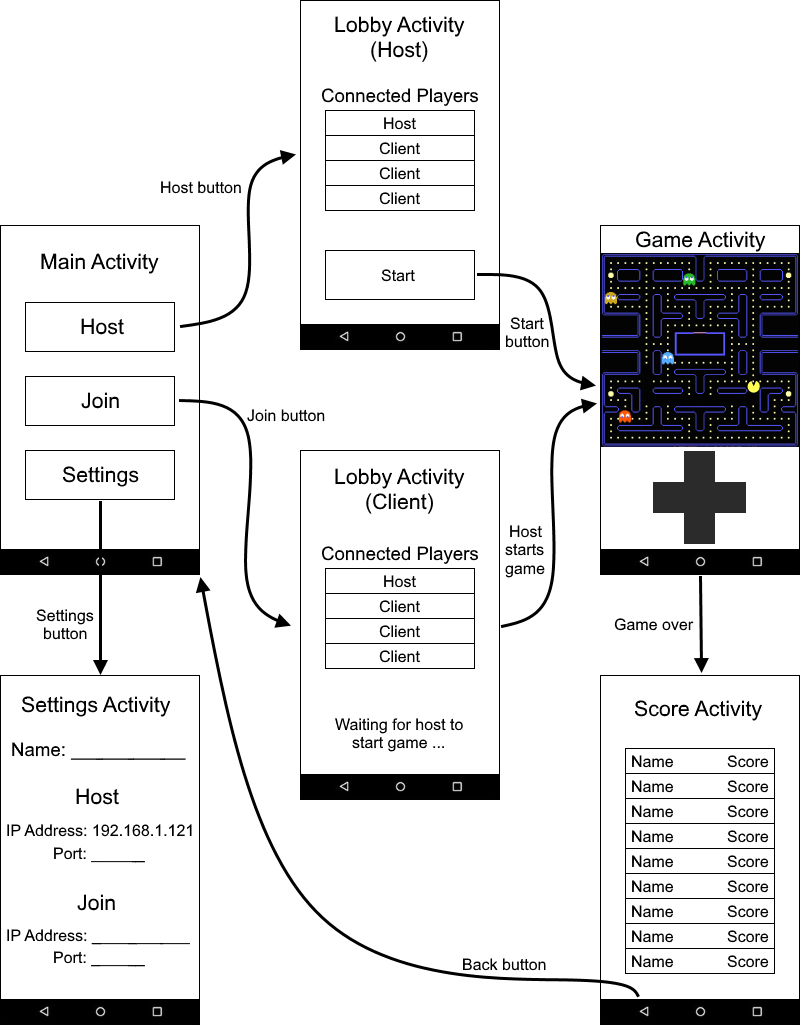
\includegraphics[width=\columnwidth]{overview.png}
    \lfig{activity-overview}
    \vspace{-5mm} % use negative white space to fix too large gaps
	\caption{Activity Overview}
\end{figure}

Figure 2 provides a raw draft of the game's architecture.

The following three threads will be used:
\begin{enumerate}
	\item Communication Thread:\\
	To prevent blocking of the UI thread, all network communication will be outsourced to a separate communication thread.
	If the device works as server (host), this communication thread will be a server thread and needs to deal with receiving and distributing network messages from multiple clients.
	If the device works as client, the communication thread only needs to send outgoing commands and receive game state.
	
	\item Model Thread:\\
	The model thread keeps track of the game state and is responsible for state updates as well as computations on the state. Furthermore this thread receives user commands provided by either the communication thread or the user interface thread.
	
	\item UI Thread:\\
	The UI thread is responsible for displaying the current game state to the user. 
\end{enumerate}


\section{Requirements}

%-------------------------------------REQUIREMENTS------------------------------------

\begin{enumerate}
	\item The game can be played on multiple Android devices (at least two).
	\item The gameplay should work as follows:
	\begin{enumerate}
		\item One player plays as Pac-Man.
		\item One or multiple other players play as ghosts.
		\item Each player figure constantly moves forward unless the movement is blocked by a wall element. This means that the only way to completely halt movement for a player is to run into a wall without changing direction.
		\item In case it helps balancing the gameplay, power-ups (objects that provide special abilities to Pac-Man or the ghosts) spawn randomly on the map. Those power-ups might improve or worsen the performance of the player figures. Power-Ups can be collected by simply moving over them.
		\item The amount of rounds played corresponds to the amount of players connected.
		\item Pac-Man starts with a predefined amount of lifes.
		\item When Pac-Man is being captured by a ghost, he loses one life and all ghosts will return to their spawn.
		\item The round ends if either all coins have been collected, Pac-Man has lost all his lifes, or the round-timer (predefined and the same for each round) reaches zero.
		\item Each player plays as Pac-Man for one round and as ghost for the remaining rounds.
		\item After all rounds have been played, the game ends and the players can see the amount of points achieved by each player.
		\item The host will start as Pac-Man in the initial round.
		\item Clients will start as ghosts in the initial round.
	\end{enumerate}
	\item Each player must use one Android device in order to control his figure (Pac-Man or ghost).
	\item The map (board) on which the players move should provide the following features:
	\begin{enumerate}
		\item Pac-Man starts on a predefined location (Pac-Man spawn).
		\item The ghosts (one ore multiple) start on predefined locations (ghost spawns).
		\item Player figures can only move up, down, left and right.
		\item The only structuring elements of the map are walls.
		\item Walls have either horizontal or vertical orientation.
		\item Player figures can not move through walls.
		\item The map has rectangular shape and is limited by walls at its borders (horizontal walls along the left and right border, vertical walls along upper and bottom border). On two ore more locations the wall on the border of the map is open and players can teleport to the other side of the map. Teleporting means that players exiting the board on the right side will spawn again on the left side and vice versa.
		\item Coins are distributed evenly on the game map (board).
		\item Every coin on the map must be reachable by all player figures. 
		\item When Pac-Man collects a coin by moving over it, the coin disappears from the map and Pac-Man receives points.
		\item The player with the most points wins the game. In case of a draw, the player that completed his round the fastest is the winner.
	\end{enumerate}
	
	\item The communication among the devices will be implemented on top of TCP (or UDP).
	\item The minimum SDK required is API 21: Android 5.0 (Lollipop). The target SDK version is API 24: Android 7.0 (Nougat).
	\item On the hosting player's device, a service will be started to run the server which the clients can connect to.
	\item As a game development engine the ANDEngine is used. This is a free Android 2D OpenGL game engine [1].
	
\end{enumerate}


\section{Work Packages}

%-----------------------------------WORK PACKAGES----------------------------------

\begin{itemize}
	\item {\bf WP1}: Define appropriate model for game situation (state) and methods to change the state.        
	\item {\bf WP2}: Design graphical representation for Pac-Man player figure.
	\item {\bf WP3}: Design graphical representation for ghost player figure.
	\item {\bf WP4}: Design graphical representation for map elements (coins, walls, unoccupied positions).
	\item {\bf WP5}: Implement Game activity that connects model and graphical representation. It should also allow the user to control its figure.
	\item {\bf WP6}: Define a communication protocol to synchronize the game's state across devices. Choose appropriate transport protocol.
	\item {\bf WP7}: Implement the communication protocol - part 1: Server.
	\item {\bf WP8}: Implement the communication protocol - part 2: Client.
	\item {\bf WP9}: Combine Game activity with the communication protocol.
	\item {\bf WP10}: MainActivity, LobbyActivity, SettingsActivity, ScoreActivity design.
	\item {\bf WP11}: MainActivity functionality:
		\begin{enumerate}
			\item Host button starts LobbyActivity with boolean intent extra "is host" set to true to then enable Start button and disable "Waiting for host to start game" text in LobbyActivity.
			\item Join button starts LobbyActivity with boolean intent extra "is host" set to false to then disable Start button and enable "Waiting for host to start game" text in LobbyActivity.
			\item Settings button starts SettingsActivity.
		\end{enumerate}
	\item {\bf WP12}: LobbyActivity functionality:
		\begin{enumerate}
			\item ListView to list all connected player (might needs to be scrollable depending on how many player we allow in one game).
			\item Host can press Start button to start game for all players.
		\end{enumerate}
	\item {\bf WP13}: SettingsActivity functionality:
		\begin{enumerate}
			\item Name EditText: default name is "Anonymous" or device name.
			\item Host IP Address TextView: Shows the device's LAN IP Address.
			\item Host Port Address EditText: Allows to change the server's port.
			\item Join IP Address EditText: Allows to change the IP Address to connect to when joining a game.
			\item Join Port Address EditText: Allows to change the port at which to connect when joining a game.
		\end{enumerate}
	\item {\bf WP14}: ScoreActivity functionality:
		\begin{enumerate}
			\item ListView (possibly scrollable) to show Highscores list. When the game ends, every player will land in the ScoreActivity, receive the list from the host and display it.
			\item The Back button returns to the MainActivity.
		\end{enumerate}
\end{itemize}

\section{Milestones}

%-----------------------------------Milestones-------------------------------------

Work package distribution: 
\begin{itemize}	
	\item{\bf Group}: WP1, WP6
	\item {\bf Stefan Oancea}: WP5, WP13
	\item {\bf Johannes Beck}: WP7-8
	\item {\bf Linus Fessler}: WP2-4
	\item {\bf Markus Hauptner}: WP9, WP14
	\item {\bf Tiziano Zaramoni}: WP10, WP12
	\item {\bf Florian Morath}: WP5, WP11
\end{itemize}
Schedule:

\begin{itemize}
	\item Week 1: In the first week, the general program structure should work. This includes menu navigation, the settings menu, the lobby, and a class for the game activity. Furthermore WP1 should be finished. 
	\item Week 2: In the second week, the game map should be drawn and the player can move Pac-Man around the map and collect coins.
	\item Week 3: In the third week, the basics of the game should already work. This includes movemet of Pac-Man and the ghosts. Collision detection and networking.
	\item Week 4: The last week should be used for bug fixing, gameplay balancing and optimizations.
\end{itemize}




\section{Additional Authors}

%-------------------------------Additional Authors---------------------------------



%-------------------------------------REFERENCES-----------------------------------

% The following two commands are all you need in the
% initial runs of your .tex file to
% produce the bibliography for the citations in your paper.
\bibliographystyle{abbrv}
\bibliography{report}  % sigproc.bib is the name of the Bibliography in this case
% You must have a proper ".bib" file

%\balancecolumns % GM June 2007

\end{document}
